\chapter{Practicals}
\section{Tutorial: Protein Data Bank (PDB)}
\begin{verbatim}
    www.rcsb.org
\end{verbatim}
\noindent This is the database that contains most of the structural information of proteins. And having said that, if someone tries to publish anything related to protein structure, it's obligatory—even before the publication is accepted—to deposit all the data, and not only the coordinates that we will speak about and we will utilize, but also all the experimental parameters, all the experimental datasets, so that they can be controlled.

\paragraph{Methodologies and Statistics}
\begin{itemize}
    \item Not all the structures that are there are accessible, but... if you see a structure there, you may try to approach the authors to get a structure that you need. 
    \item Now, also it's interesting to see just for a second that the kind of the proportions, the contributions of the different methodologies are changing with the time. You can see, for example, the yellow line, the cryo-EM methodologies; they are rapidly increasing. So people are more and more interested in large protein machines. Okay, but still on the top, still X-ray crystallography, so the static structures.
\end{itemize}

\paragraph{PDB Identification Codes}
All the PDB structures that are deposited are identified by four-character codes that can be numbers or letters—of course, letters only of the English alphabet. In this case, I give you the code and this is 1JSU.

\paragraph{Analyzing a Protein Complex (1JSU)}
 We are looking at here a complex that basically consists of three proteins, okay: P27, cyclin, and CDK2.
 \begin{itemize}
     \item First, you want to make sure that the proteins that are inside are really your proteins. Go down kind of to the middle of the page where it says "Macromolecules." And then here, in the Macromolecules section, you have the chance to see... you see here molecule name, which you may not understand... but there is a code here, and this code—P24941—will unambiguously identify this protein.
     \item chain means that these are covalently bound amino acid residues, and when chain ends, the covalent bond ends as well. Okay, so this means that these are distinct, disjoint segments of protein, and whenever you would like to set up a simulation, you need to deal with them separately.
     \item And each of them, please note, they possess a UniProt number, and this number usually you write down. This is something important.
 \end{itemize}

\paragraph{Heteroatoms and Small Molecules}
\begin{figure}[h!]
    \centering
    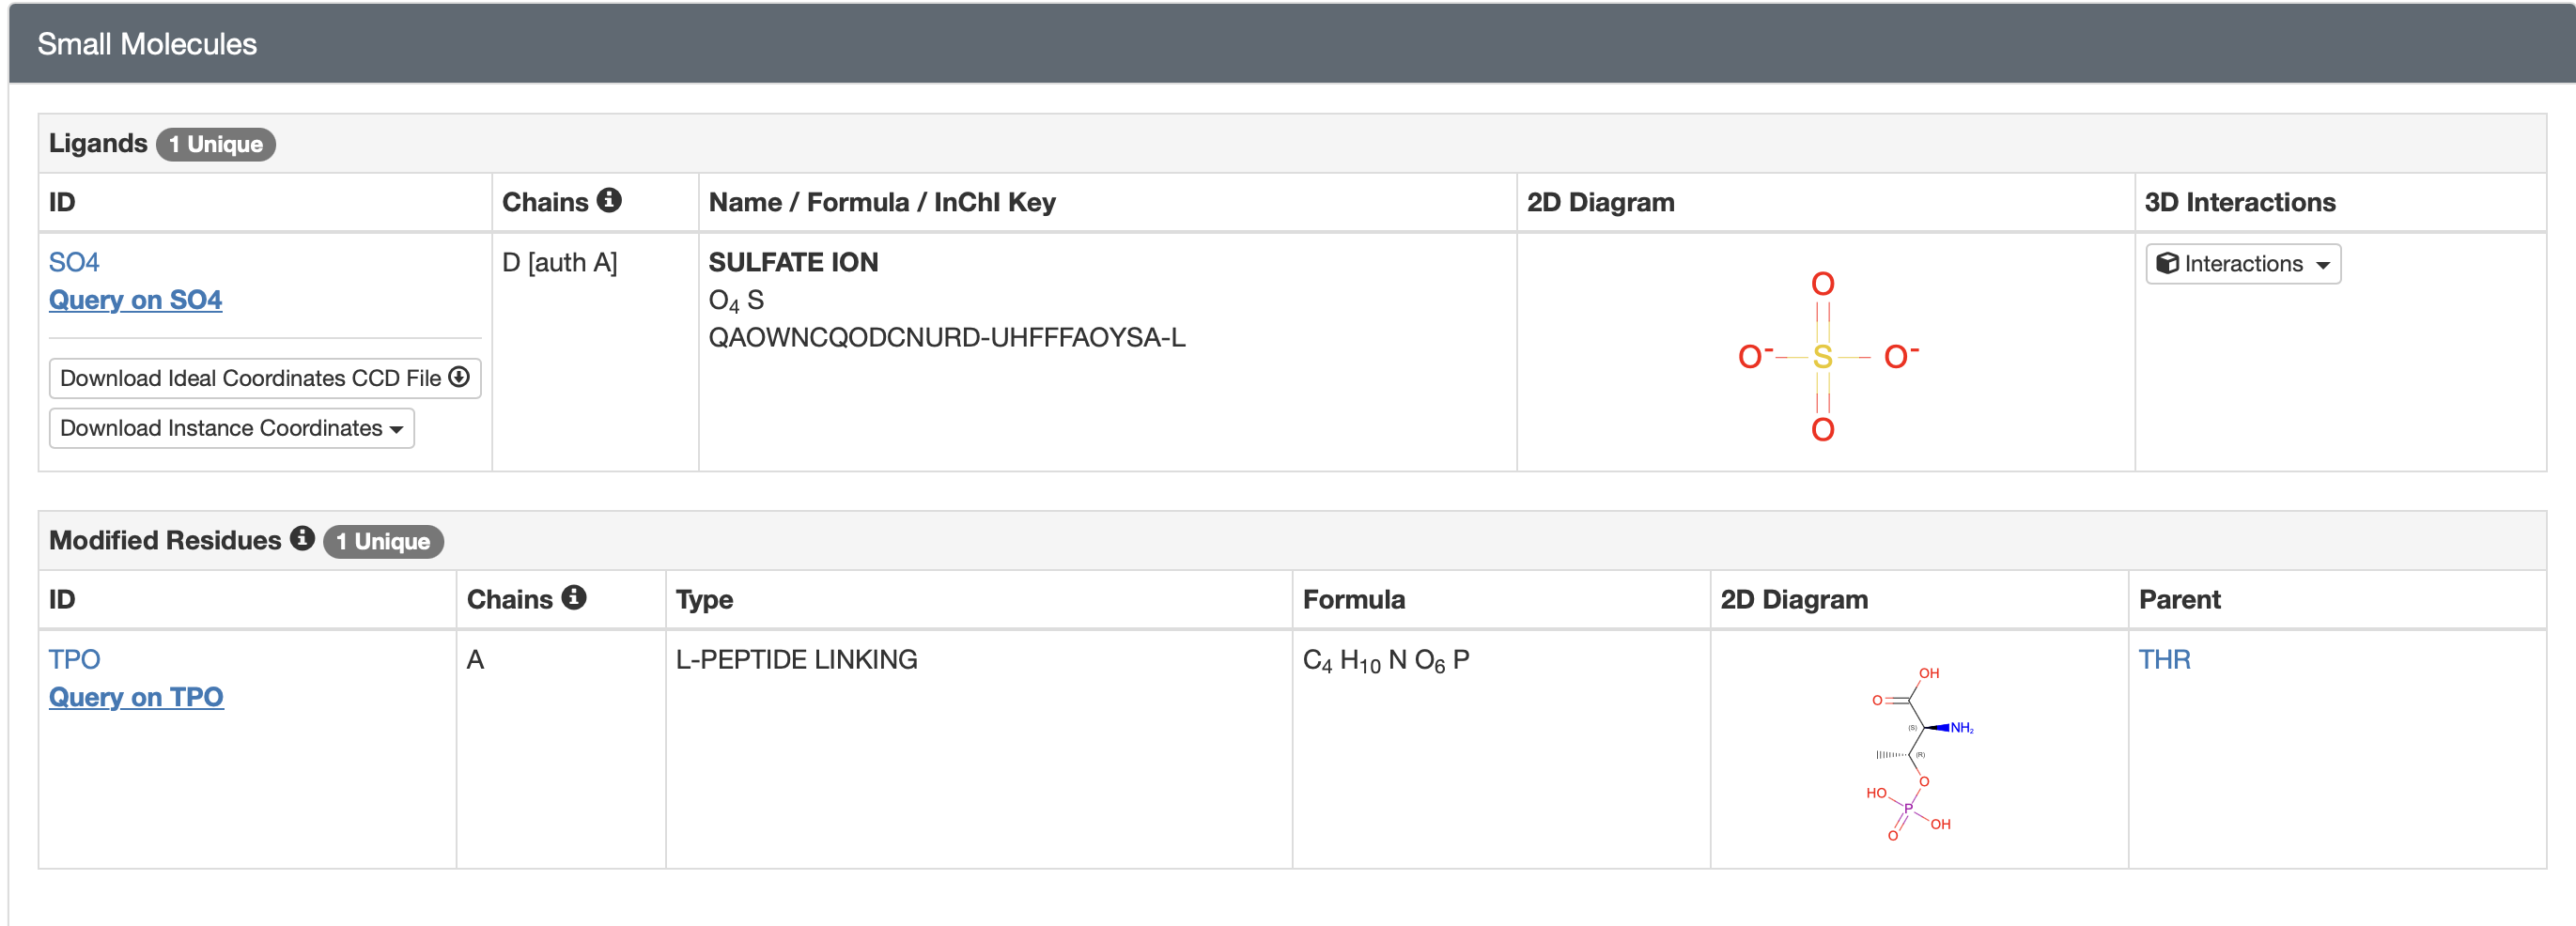
\includegraphics[width=\linewidth]{practicals_img/pdb_small_molecules.png}
    \caption*{}
    \label{fig:placeholder}
\end{figure}
If we go a little bit further, we may be interested in other issues, which means small molecules. You will see later that they are in a separate section, and each of the lines that contain these small molecules begins with a different kind of identifier. Normally the biomolecules like protein, DNA, or RNA, they start with a simple word "ATOM," where this one starts with the word "HETATM," which means heteroatom. Now why do we care, why do we care about these small molecules? We do care because they may be important for the functionality of the protein; they may be cofactors that may be something that are functionally required. Or here, for example, there is a residue which is a post-translational modification... this is a phosphate group. This is a threonine residue and it's phosphorylated. 

\paragraph{Sequence and Structure Correspondence}
There is another issue that you need to look at: if you go to the very top of this page, you find this let's say tab which says "Sequence." Please push it. There is a sequence of the protein and this is encoded with this number. However, if the protein has a region which is disordered—either the C-terminus, N-terminus, or even in between - then it is possible that the experimentalists don't see the whole structure. So it is possible that you have a protein of 400 residues, but what is represented in the PDB file maybe it's only 300 residues or 200 residues. UniProt is the reference database for all the sequences. Look at chain B. Here we are talking about residues that come between 1 and 260, but in fact, in the UniProt sequence, you see that it's starting at 173. So when you search for identity of residues, this is something that is really critical.
\begin{figure}[h!]
    \centering
    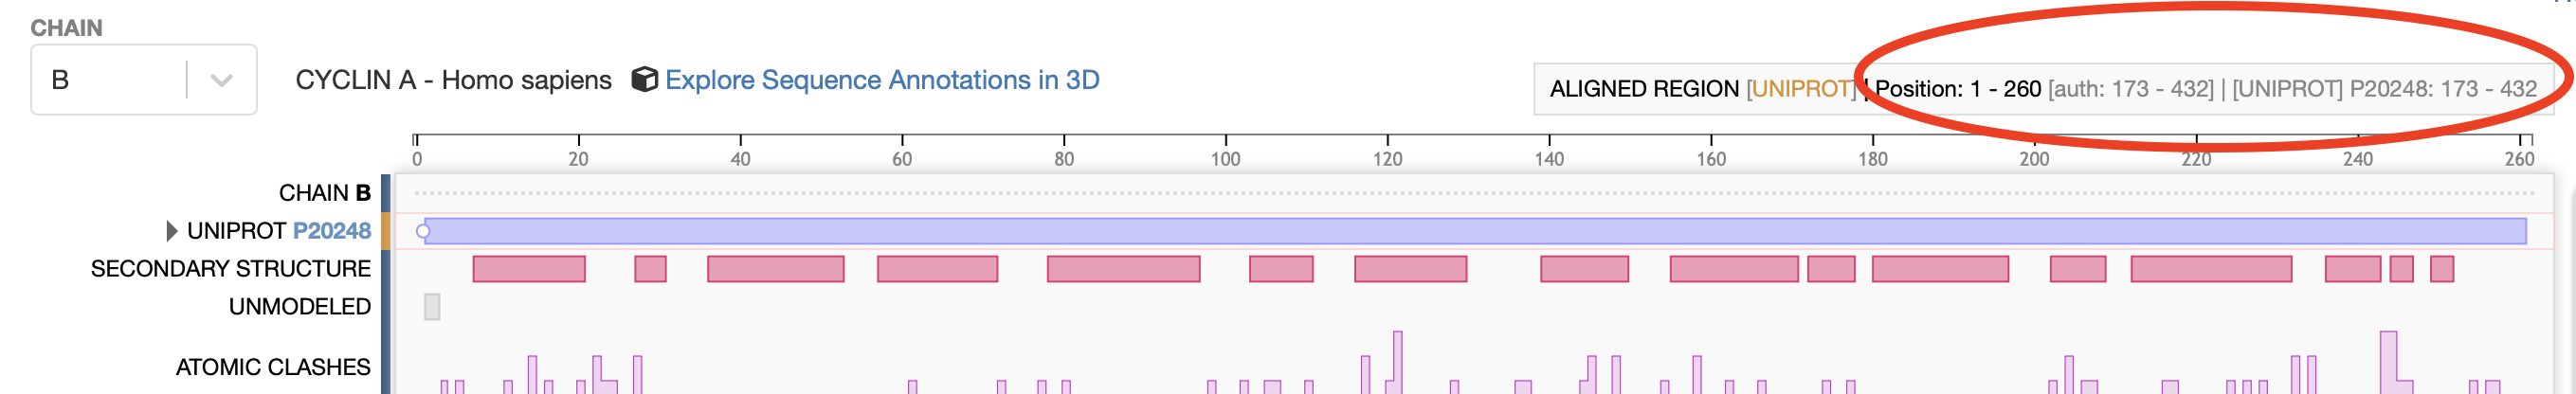
\includegraphics[width=\linewidth]{practicals_img/pdb_alignment.png}
    \caption*{}
    \label{fig:placeholder}
\end{figure}

\paragraph{Exploring the PDB File Header}

\begin{figure}[h!]
    \centering
    \includegraphics[width=\linewidth]{practicals_img/PDB_GLYCINE.png}

    
    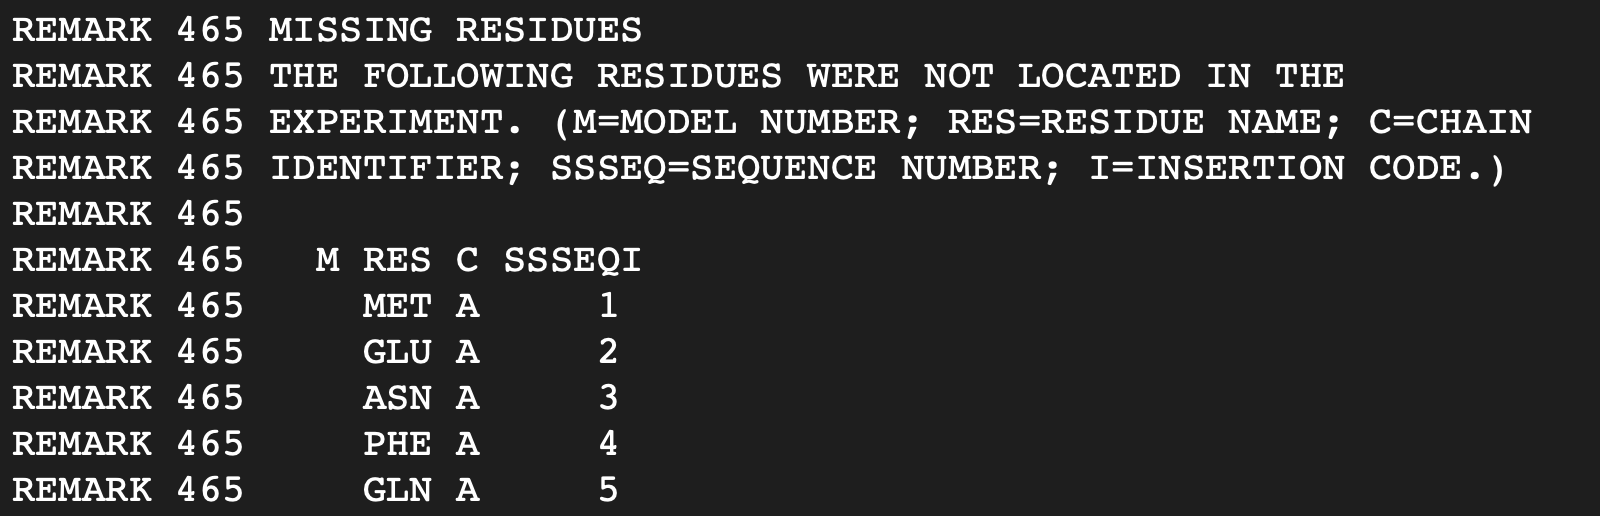
\includegraphics[width=\linewidth]{practicals_img/pdb_remark_missing_residues.png}
        \caption{TOP: Hydrogen atoms are not reported. In this example: a glycine amino-acid. BOTTOM: the missing residues remark, in the file header.}
    \label{fig:placeholder}
\end{figure}

Download the legacy PDB file. At the start of the file, there are many things that you may be interested in, which you can also get from the structure article. What things you may be interested in?  You may be interested in: from which organism your molecule was expressed expressed for the structural analysis. Here, for instance, it was expressed in the E. coli. It may be important because, for example, \textbf{in the bacteria there is no phosphorylation}. So, if you use a human protein which has an important phosphorylation site, for example, you would lose it in the final structure. Sometimes they report a remark on missing residues if they couldn't determine a position of a few residues... then you should know what to do with these. This may also appear as disorder in the original PDB file. Unfortunately, this is not the case. Because there are some long residues, long side chains, that may be very mobile. And in that case, researchers may not see the end of it. And very unfortunate... and we will see some of the long residues, for example the positively charged residues, the lysine or the arginine. And unfortunately, if they don't see the last residues, the last groups, the atoms... by the way, only the heavy atoms, because we are talking about crystal structures...

\paragraph{The ATOM Records}


\begin{itemize}
    \item \textit{Column 1}: Contains "ATOM" for atoms belonging to the polypeptide chain, "HETATM" for the small molecules outside of the chain and the water molecules captured.
    \item \textit{Column 2}: An arbitrary  consecutive numbering. Totally ignorant if something is missing from the structure.
    \item \textit{Column 3}: Codified atom names (e.g. CA is the alpha carbon).
    \item \textit{Column 4}: Codified three letter residue identifier.
    \item \textit{Column 5}: Chain identifier. It is a letter, although not necessarily A or B or C —  depends on the authors.
    \item \textit{Column 6}: Residue number. This is a number in the structure; this may NOT correspond to the number of the residue in the reference sequence file (UniProt). It is possible that the experimentalists list two residues as consecutive whereas  in the real protein there is a ten-residue gap between the two. Therefore, it is always good to cross-check with the UniProt sequence.
    \item \textit{Column 7,8,9}:Coordinates xyz,
    \item \textit{Column 10}: this number is almost always one, unless the structure has undergone a very special experimental method or anomalous refinement, when they present kind of two conformers for each of the atoms. It's possible and then the one become half and half, so this basically tells you the occupancy.
    \item \textit{Column 11}: the B factor. This is related to the thermal motion of the atoms. Normally, when they do the refinement, when they kind of a little bit adjust the experimental data with the help of some very primitive simulation methodology, they normally use isotropic refinement assuming that isotropic motion of the- of the atoms. If they are performing more sophisticated methods or high resolution, then you may find some secondary lines with different numbers talking about anisotropic refinement and motions to- to different directions. Now, what is the meaning of this? We will kind of represent these B-factors later. So this tells you something about the mobility, but it's not just strictly the mobility. Don't forget these are experimental evaluations of experimental data, so this is also kind of taking up some of the errors. When you find—when you see these numbers like here, I don't know, like in the 20s, 50s, it's all very fine. However, when you start seeing these numbers high—80, 90, sometimes it's even 100 and touching the previous column—it means that there is a problem there, there is too large mobility there, so that's kind of a suspicious part of the structure that you may have a look at.
\end{itemize}

\section{Tutorial: PyMol visualization of the $1$JSU protein (PDB entry)}

If you want to create a new selection group for a specific chain (e.g., Chain A):

\begin{verbatim}
select my_chain, chain A
\end{verbatim}

If you want to change the actual name of some object in the menu:

\begin{verbatim}
set_name old_name, new_name
\end{verbatim}



Now, the philosophy of PyMOL is that you show everything until you don't say hide. So you know, you can display several options and then for particular subsets, whatever, you can just say hide, okay? Until you don't say hide, it will be all on the screen, okay?

The label option which is here is the least used, let's say, because it's not let's say it's not so good for publication quality, but the it may orient you in one way or another so temporarily you can- you can label your residues, for example, three letters or one letter or whatever. And color, this is what you use probably most frequently because you want to distinguish between the different parts of your protein.

So I'm trying to accelerate now. I have this structure and well we said it contains three molecules but have no idea. If I color, normally I look for, you know, where the enter, where the molecule starts, when does it end. So I- I put—I click on color and there are options like spectrum and I just choose rainbow. If I choose this rainbow something, what it will do for me, it will color very dark in the very beginning of the molecule which is here until red which is the- which is the very C-terminus.

However, again, I have three molecules here. How do I- how do I know? Well, there are two ways. One is that I remember from the PDB that I had and I can type this command for example, sel chain A, just very simply. And this will be chain A, okay, and you see here it selected all, it replaced how many atoms are selected. And either in the action, I can- I can rename it. It's good to rename it and I don't rename it as chain A, can rename but I- I remember it was CDK2, this was a molecule name and that's useful to rename it as the molecule name. So I rename it as CDK2.

I can do the same, then I- you need to click out because also until you don't click out, everything is kind of added. So you need to click out of this. And you can also select in the same way, let's say, select chain B, but you can—I put into the PDF file there is—it's selection alphabet area, you can choose residues from this to this, only atom C alpha, so I mean it's a real programmable language, okay? I- I'm just showing you the very first baby steps once you feel it you can program it.

So you can select chain B and you can also change the naming in the command line, you can say set name set—first when select it's called sel and change it to cyclin. And then I have another subset which is called cyclin. At this stage it's useful to save the session, to- at the top you can say file, save session as, and maybe update class practical or whatever, and from then on don't- don't forget saving.

Okay, there is a third way how to select the subsets and this may be useful. So if you—maybe in your screen is not the right bottom but you find the letter which is called S. And this S letter corresponds to the sequence. So if I click on it, I should get a long series of letters with all the sequence here and if I observe it carefully, it's listed here A, and then if I scroll it somewhere it's listed B, and so on.

So even I could do my selections here if I didn't want to, you know, use command line or whatever. There are lots of—I mean, these one-letter code, even if you don't—if you have not learned them but you know they signify amino acids. Then have lots of O O O, this means they are water molecules.

Okay, we will undisplay water molecules because for the moment we- we don't want them to be seen and you can just say here all hide and you look for waters. And I undisplay them, so it's, you know, cleaner. Later on, I can display some of these water.

So anyway, we can go to chain C here and I can scroll it and with the shift bar I can go until the end of it and this will be my chain C, the third molecule, which was called in the PDB file p27. So that's great. I have now, I save my session, I have now the three molecules, but it's not a very meaningful coloring.

I should see—but I prefer seeing these three molecules as—with different colors based on the subunits, let's do this first. So does every—does everyone have the- the subsets? Is everything okay? Franco? Is everything okay? No questions?

Speaker 2: No questions now.

Speaker 1: Okay, perfect. So then you can come here CDK2 color and you choose whatever color you like. I will tell you why I choose grey. I will just choose grey 70.

And then for the other, for the cyclin, I will also choose grey but I choose a darker one, maybe grey 40. And at this point it's very useful to change the background color, which you can change here display or the very—so this is the very top menu, you have several options for- for the display and here you can change the background and I will just change it to white.

Okay, and I turn it a little bit. There is another feature which people who have some problems with vision may utilize. There is something like depth cue or fogging. If you switch it off, you- you have less 3D dimensionality but just as a—just as a display but you have stronger colors. I usually use it.

You see it's—so this is actually quite nice. You can adjust this display setting. For example, this you can see the helices, you can see some beta strands and some of these loops are very thin. So there are all kinds of options to change it. For example, I can say set cartoon loop radius, okay, and I give a number, maybe 0.4 or something. Ah, I- even I made a mistake. Okay, I hope it's okay... yes, it accepted.

So you see that everything has grown. But you can change everything, you can change the look of the helix, you can change separately for the beta strands, so you can, you know, you can play around with it. So in this manner, for example, I save—by the way I save the session. Okay, I can start seeing how this is constructed from three molecules. Two are kind of making the unit and one is kind of around.

Now what is around is an inhibitor. So let's do as follows. Let's display this whole thing as a surface and let's- let's see the overall organization. So we go to the S button here in the- in command and we say show surface.

And this is quite nice. First of all, you can see how rugged the protein surface is and you can see the kind of a hug that this little red gives to the other two proteins. But this kind of a hug inhibits cell cycle to go on and when this kind of hug is- is removed in one way or another, then the cell cycle continues. So this is an important hug.

Now this is very nice and I suggest, you know, you can send it to your beloved ones on 14th of February, but this is not so useful if you want to do computational analysis. Because in principle, you want to see how the hug occurs, which residues interact with which other residues, okay?

And for that matter, it would be useful to- to undisplay the- the surface for the p27, the red one. So I would hide the surface, okay, just for this one, and then see how it interacts with the others. But there is still a problem here—of course there are always problems, but we create and resolve them. So you can see that there are some holes, right, on the surface of the other two molecules. Obviously because it would be the place for the surface of p27.

\begin{figure}
    \centering
    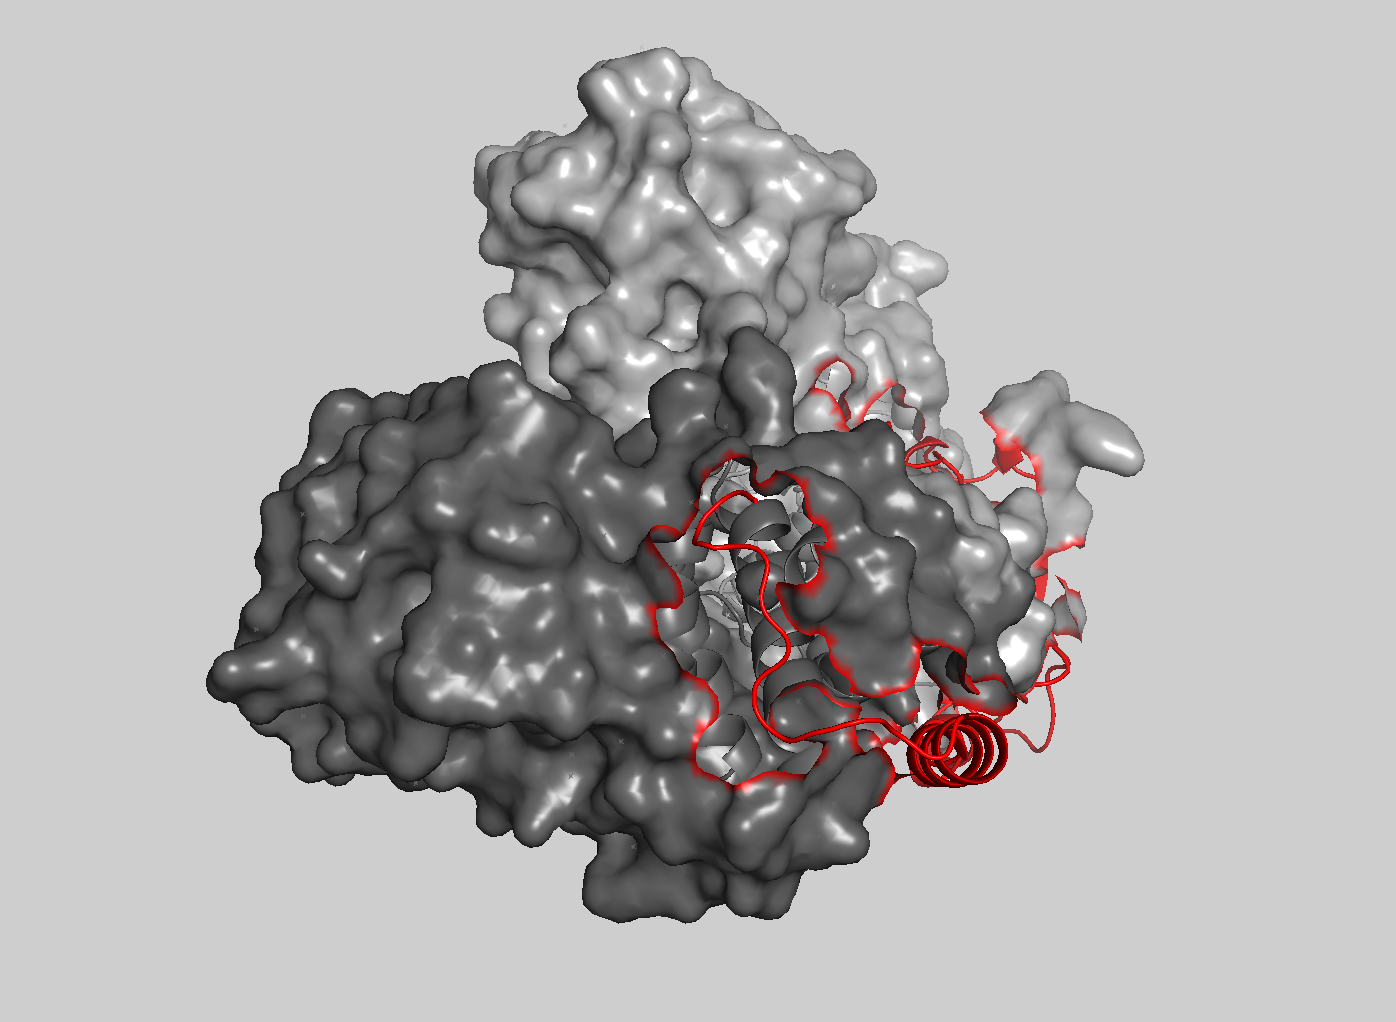
\includegraphics[width=0.45\linewidth]{practicals_img/pymol_surface_problem.png}
    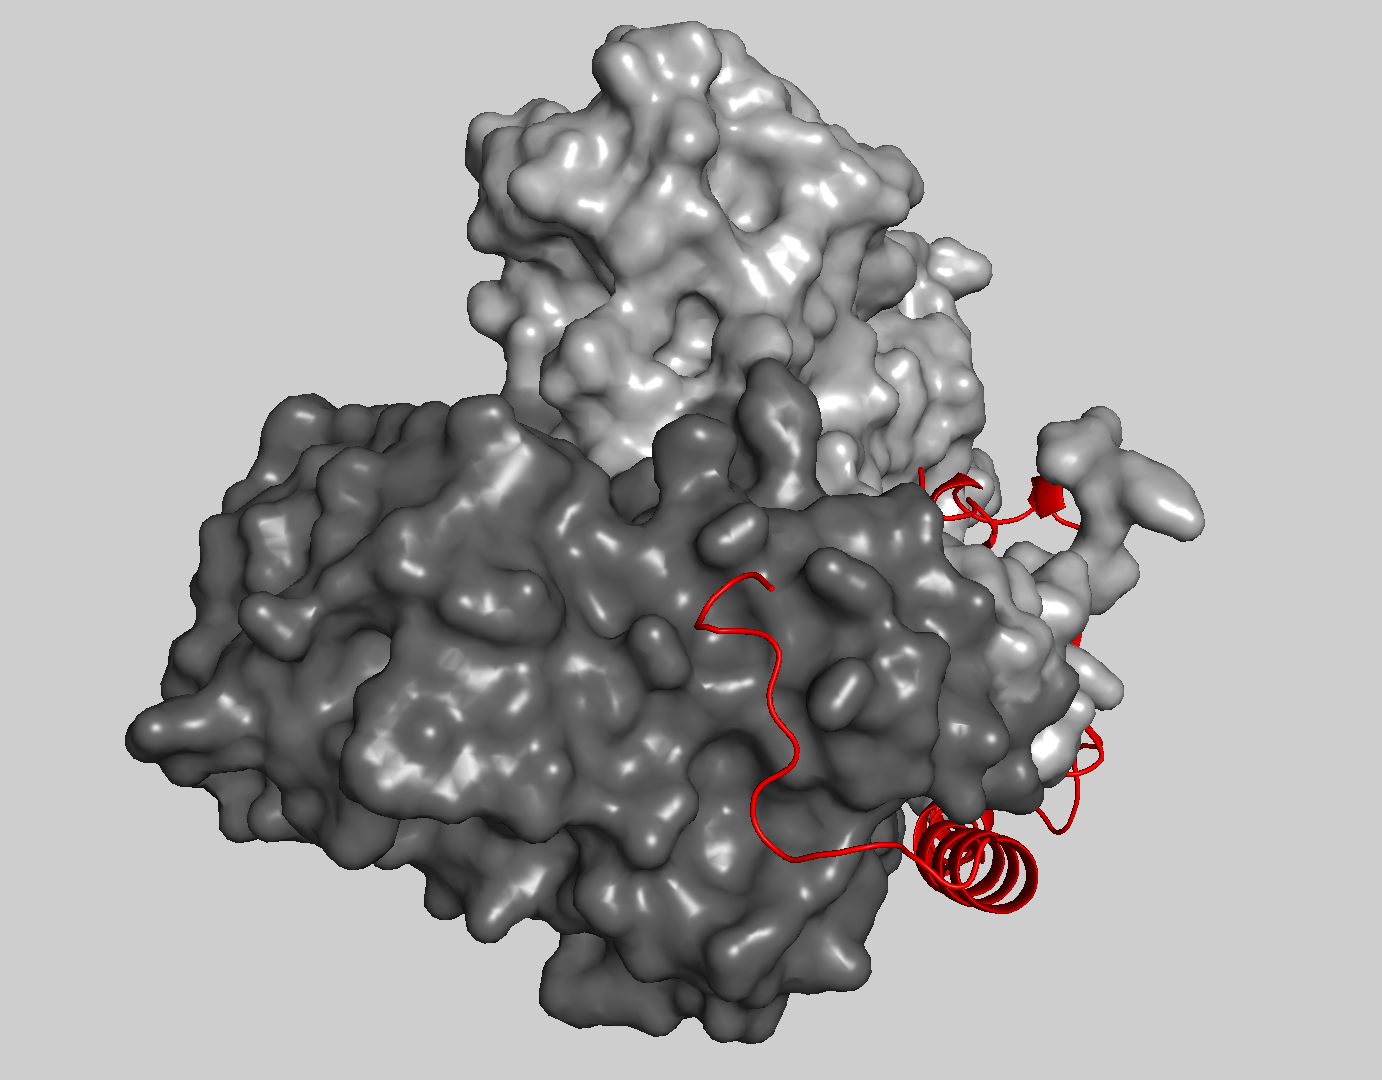
\includegraphics[width=0.45\linewidth]{practicals_img/pymol_surface_solved.png}
    \caption{Caption}
    \label{fig:placeholder}
\end{figure}
So to solve this kind of problems, I posted another structure. Basically what you need to use is to generate the structure which contains only chain A and chain B, so only the two grey ones, okay? And then you basically take a- you- you read that in. I'm just showing to you now, but you can repeat it at home.

So you can open my file that I posted for you and this is—I'm sorry, uh... yes, so it is called CDK2 cyclin. So this is without the p27. I read in that file, you can see already there is another file. If I hide for the second the- the surface, you should see that I have a file somewhere, maybe it's centered in another part. And basically I can just say—and all of these are listed in your PDF files—align this CDK2 cyclin on the 1GSU.

And once you do this, this is a rigid body alignment, so rigid body rotation and translation. You see already that this kind of cyan color appeared and you see here that the root mean square deviation is zero. Because it's zero because it's basically the same structure. Unfortunately to make a very nice image, I would quickly need to do the same thing, which instead of typing I would just do here. So I need to—I need to define the two sets of the CDK2 here... okay.

So I need to define in order to generate the same picture, I will just call now chain A and chain B, but you can call in whatever way you want. Okay... okay. Okay. I color these in the same way how it was colored before. Okay.

And I undisplay everything, the CDK2 and the cyclin from the previous structure. I undisplay, hide, hide, and I also hide everywhere the waters. So in that manner now I have a composite structure. And if I say now to show the surface for this cyclin structure, which doesn't know in principle about the p27, you can see that this is your first nice image. Okay, I also posted the images in your Moodle so that you can play around with them. This is the first place when you can start feeling how this is anchored here, how this is anchored here and so on.

So let me tell you now in a few words what are the next following steps that you can do. First to save your session. Now if you are pleased with the image, you can just go to this ray or draw and you can adjust to your DPI and you can just say ray. And you can save the image and this image will be saved in a manner—okay, I imitate here—will be saved in a manner that will be completely transparent in the background.

Speaker 2: We cannot see the settings for the background ray.

Speaker 1: You cannot see. Then in the academic maybe you cannot do this, but anyway if you save the image you should be able to ray it and you should be able to get the image with a transparent background. And when you read it into any kind of program, Word or PowerPoint or whatever, I mean you can all put something on the background. When I save the image, whatever name, I just call it class image. Okay, once I saved it, if you click on it, it becomes to your original image and so on.

So this is kind of just the very beginning of the beautiful story. So let me tell you now in a few words what comes after it and you will continue now with Franco who- who can show you how to really compute with it. But you need to be able to tackle it. So in a few minutes, I- I tell you what else you can do.

So this is a very nice story of this cell cycle inhibition and there are some competitors here, there are some viruses which can imitate, so there is a third PDF file in your Moodle section that tells you the whole story, that tells you many other structures, how it comes, how one replaces another, how you search because the next step would be how you search for the motifs that are contacting each other. Then you can, you know, see whether it's in the mobile part, not mobile part, is hydrophobic, not hydrophobic.

So the play starts from here. There are many, many things that you can do—identifying residues that are in contact, or for example you try to show—sorry—you try to show for example the B-factors, which are the mobile part, which are the fixed part. You can see that it's relatively rigid when it touches and so on. So you can do all this kind of games and they are all in the PDF files.

The second step that you can do and we will do with Franco with BioPython that you find three structures...


